\documentclass[11pt]{article}         

\usepackage{amsmath}
\usepackage{flafter} 
\usepackage[paper=letterpaper,margin={1.5in,1.5in}]{geometry}
\usepackage{graphicx}
\usepackage{microtype}
\usepackage[round,sort]{natbib}
\usepackage[section]{placeins}
\usepackage{rotating}
\usepackage{setspace}
\usepackage{tocbibind}
\usepackage{url}
\usepackage[pdfborder={0 0 0}, bookmarksnumbered=true, colorlinks=true,
	linkcolor=blue, urlcolor=blue, citecolor=blue]{hyperref}

\bibliographystyle{abbrvnat}

\title{Technical Manual for SigmaSpectra}
\author{Albert R. Kottke and Ellen M. Rathje}
\date{\today}

\begin{document}
\maketitle
\tableofcontents

\onehalfspacing

\section{Introduction}

SigmaSpectra is a computer program that selects suites of of earthquake ground
motions from a library of ground motion such that the median of the suite
matches a target response spectrum at all defined periods, and then scales the
suite such that the standard deviation agrees with the target standard
deviation. The success of the SigmaSpectra in matching the target response
spectrum and standard deviation depends on many factors including: the size of
the requested suite, the number of motions in the ground motion library, and the
appropriateness of the target response spectrum and standard deviation to the
motions in the library.

SigmaSpectra is distributed under the GNU General Public License version 3
(GPLv3) which can be found here: \url{http://www.gnu.org/licenses/gpl.txt}, or
in the installation directory of SigmaSpectra. As part of the GPLv3 license the
source code has been made available in the installation file.

\section{Methodology}\label{sec:method}

The methodology for the scaling of the ground motions used in SigmaSpectra is
published in \citet{kottke:07} and \citet{kottke:08}. The major limitation of
SigmaSpectra is the complete reliance on the response spectrum for the
selection. Therefore, aspects of the ground motion that are not captured in the
response spectrum are ignored during the selection and need to be selected by
the user. The user interaction within the selection process occurs during: the
development of the ground motion library (see Section~\ref{sec:example:library},
the optional step of flagging motions, and the final selection of a ground
motion suite.

SigmaSpectra uses a two step process for selection and scaling. Suites of
motions are first selected from the library to match the target response
spectrum. The suite motions are then scaled to match the target standard
deviation while maintaining agreement with the target response spectrum.

\subsection{Basics of Scaling}\label{sec:method:basics}

SigmaSpectra computes the scale factor adjust the amplitude of a ground motion and does
not modify the frequency content in any manner.
A suite of scaled response spectra are typically assumed to be
log-normally distributed. Therefore, the median spectral acceleration of the
scaled suite ($\overline{S}_a^\text{scaled}$) at the $i$-th period is found
by computing the mean log-space:
\begin{displaymath}
	\ln \overline{S}_a^\text{scaled}(i) = \frac{1}{n_m} \left[ \ln\left( s_{1}
	\cdot S_{a,1}(i) \right) + \ln\left( s_{2} \cdot S_{a,2}(i) \right) + \dots
	+ \ln\left( s_{n_m} \cdot S_{a,n_m}(i) \right) \right]
\end{displaymath}
where $n_m$ is the number of motions in the suite, $s_n$ is the scale factor of
$n$-th motion, and $S_{a,n}(i)$ is the spectral acceleration of the $n$-th motion
at the $i$-th period. Using the properties of logarithms the average response
spectrum can be expanded to:
\begin{multline*}
	\ln \overline{S}_a^\text{scaled}(i) = \frac{1}{n_m} \underbrace{\left[ \ln
	s_1 + \ln s_2 + \dots + \ln s_{n_m} \right]}_\text{Controls Amplitude} \\
	+ \frac{1}{n_m} \underbrace{\left[ \ln S_{a,1}(i) + \ln S_{a,2}(i) + \dots + \ln
	S_{a,n_m}(i) \right]}_\text{Controls Shape}
\end{multline*}
The expansion shows that the scale factors control the amplitude of the median
response spectrum while the motions that make up the median response spectrum
govern the shape. The expansion can be further simplified to:
\begin{displaymath}
    \ln \overline{S}_a^\text{scaled}(i) = \frac{1}{n_m} \sum_{j=1}^{n_m} \ln s_j +
	\frac{1}{n_m} \sum_{j=1}^{n_m} \ln S_{a,j}(i) = \ln \overline{s} + \ln
	\overline{S}_a(i)
\end{displaymath}
This equation shows that the amplitude of the median response spectrum  of a
suite is controlled by the average of the scale factors ($\overline{s}$).
Furthermore, the individual scale factors can be changed without affecting
$\overline{S}_a$ as long as the average remains the same.

The optimal average scale factor ($\overline{s}$) for a suite of motions can
be found by:
\begin{displaymath}
	\ln \overline{s} = \frac{1}{n_p} \sum_{i=1}^{n_p}\left[ \ln\left(
	S_a^\text{target}(i) \right) - \ln\left( \overline{S}_a(i) \right) \right]
\end{displaymath}
where $n_p$ is the number of periods in the response spectrum. This average
scaled factor represents the least-squares fit of the median response spectrum
spectrum.

\subsection{Selecting Motions}\label{sec:method:selecting}
Before discussion of how suites of ground motions are selected, it is necessary
to define a measure of the goodness of fit that can be used to compare two
different suites. SigmaSpectra uses the root-mean-square-error to quantify the
goodness of fit, and is computed by:
\begin{multline*}
	\text{RMSE} = \sqrt{\frac{1}{n_p} \sum_{i=1}^{n_p}\left( \ln
	\overline{S}_a^\text{scaled}(i) - \ln S_a^\text{target}(i)\right)^2 } \\ =
	\sqrt{\frac{1}{n_p} \sum_{i=1}^{n_p}\left( \ln \overline{S}_a(i) + \ln
	\overline{s} - \ln S_a^\text{target}(i)\right)^2 } 
\end{multline*}
When selecting motions, the optimal scale factor ($\overline{s}$) is first
computed, and the RMSE of the suite is computed.

The most rigorous method for selecting a suite of ground motions would be trial
of every possible combination. However, depending on the size of the motion
library and the required size of the suite, the time required to test each of
the trials may be prohibitive (e.g. days to weeks). An alternative approach
would be to select a seed motion, and then try each of the remaining motions.
Adding the motion  that results in the lowest RMSE to the suite. This process
is repeated until the desired suite size is achieved. However, this approach
suffers from not trying enough combinations.

SigmaSpectra uses a hybrid approach in which the seed combination is generated
for a given seed size, and then the iterative approach is used to select the
remaining motions. This allows for the number of trials to be tuned by changing
the seed size. The rigorous trial of every possible combination can be achieved
by setting the seed size to the suite size, or a suite can be built for each
motion as a seed motion by setting the seed size to 1.

\subsection{Scaling a Motion Suite}
Consider a normal distribution, that is separated into four equal area
(probability) sections. The centroid of each section is found and represents the
expected value within the section. For example, four centroids for standard
normal distribution ($\mu=0$ and $\sigma=1$) are located at -1.275, -0.325,
0.325, and 1.275. The standard deviation of these values is 0.93, just below the
target standard deviation. At a centroid location ($\varepsilon_i$), the target
response spectrum for the centroid is computed by:
\begin{displaymath}
	\ln S_a^\text{centroid}(i) = \ln S_a^\text{target} + \varepsilon_i \left( \beta
	\sigma_{\ln}^{\text{target}} \right)
\end{displaymath}
where $\beta$ is an scale factor that adjusts standard deviation of the target
standard deviation.  The motions in the suite are sorted based on the mean
response over all periods, where the mean response of the $j$-th motion is
defined as:
\begin{displaymath}
  \overline{S}_{a,j} = \frac{1}{n_p} \sum_{i=1}^{n_p} \ln S_{a,j}(i)
\end{displaymath}
The motion corresponding to the smallest $\overline{S}_{a,j}$ is 
fit to the centroid curve computed by the smallest $\varepsilon$
value (e.g., -1.275) using a least-sum-of-squares fit. The same technique is
used for each of the remaining motions in the suite. This ordered scaling is
used to reduce the relative size of the scale factors (i.e., low intensity
motions stay relatively low, high intensity motions stay relatively high).

The suite generated with these scale factors may not be the best fit to the
target response spectrum. The standard deviation typically exceeds the target
standard deviation because of the added variability of each motion. To solve
this problem, the standard deviation scale factor $\beta$ is adjusted from 0 to
3 and the scale factor that results in the best fit to the target standard
deviation is selected. The goodness of fit for the standard deviation is
measured by the root-mean-square error, defined by:
\begin{displaymath}
	RMSE_{\sigma_{\ln}} = \sqrt{\frac{1}{n_p} \sum_{i=1}^{n_p}\left(
	\sigma_{\ln}^\text{suite}(i) - \sigma_{\ln}^\text{target}(i) \right)^2 } 
\end{displaymath}

\section{SigmaSpectra User Interface}

This section introduces the SigmaSpectra user interface and provides information
regarding each input field.

\subsection{Input Dialog}

After launching SigmaSpectra, the Input Dialog, shown in
Figure~\ref{fig:interface:inputWindow}, is created and contains all of the
parameters used in the selection process. The Input Dialog is separated into the
following four groups:
\begin{enumerate}
  \item Target Response Spectrum (Section~\ref{sec:interface:target})
  \item Period Interpolation (Section~\ref{sec:interface:periodInterpolation})
  \item Library of Motions (Section~\ref{sec:interface:libraryOfMotions})
  \item Calculation (Section~\ref{sec:interface:calculation})
\end{enumerate}
The input fields within each group are discussed in the following subsections.

\begin{sidewaysfigure}[h]
  \begin{center}
	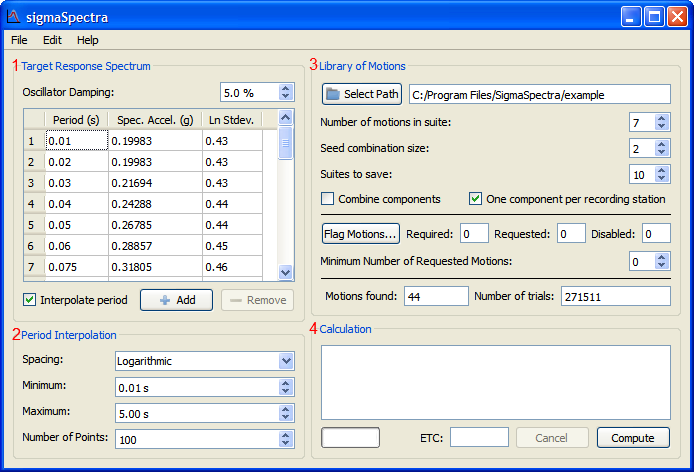
\includegraphics[scale=0.7]{screenshots/inputWindow}
  \end{center}
  \caption{Screen shot of the Input Window.}
  \label{fig:interface:inputWindow}
\end{sidewaysfigure}

\FloatBarrier
\subsubsection{Target Response Spectrum Group}
\label{sec:interface:target}

\begin{figure}[h]
  \begin{center}
	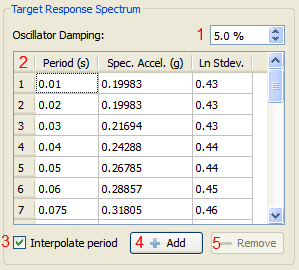
\includegraphics[scale=0.7]{screenshots/targetResponseSpectrum}
  \end{center}
  \caption{Screen shot of the Target Response Spectrum Group.}
  \label{fig:interface:targetResponseSpectrum}
\end{figure}

The Target Response Spectrum Group is used to define the target response
spectrum, and consists of three input fields. The fields are numbered in
Figure~\ref{fig:interface:targetResponseSpectrum}, and described as follows:
\begin{enumerate}
  \item The oscillator damping of the target response spectrum. This value is
	typically 5\%.
  \item The target response spectrum characterized by the spectral acceleration
	($S_a$) and standard deviation ($\sigma_{\ln}$) at a range of oscillator
	periods. The values must be specified with increasing oscillator periods.
	Rows can be added to the table by pressing the \emph{Add} button (\#4 in
	Figure~\ref{fig:interface:targetResponseSpectrum}), or removed by first
	selecting the row and then pressing the \emph{Remove} button (\#5 in
	Figure~\ref{fig:interface:targetResponseSpectrum}). A row is selected by
	selecting all three cells in a row, or by clicking on the row number button.
	The complete table can be selected by clicking on square button in the upper
	left corner of the table (\#2 in
	Figure~\ref{fig:interface:targetResponseSpectrum}). The easiest way to enter
	information into this table from a spreadsheet is copying the data from the
	spreadsheet, selecting the table, and pasting the data into the table. The
	paste action can be activated through the \emph{Edit Menu}, or through the
	shortcut \emph{Ctrl+v}.
  \item This check box is used to control if the target response spectrum is to
	be interpolated. The interpolation is done using a cubic spline and may not
	be appropriate for target response spectrum with abrupt changes (e.g., an
	IBC response spectrum).
\end{enumerate}

\FloatBarrier
\subsubsection{Period Interpolation Group}
\label{sec:interface:periodInterpolation}

\begin{figure}[h]
  \begin{center}
	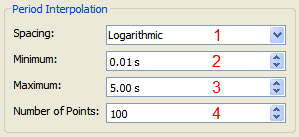
\includegraphics[scale=0.7]{screenshots/periodInterpolation}
  \end{center}
  \caption{Screen shot of the main Period Interpolation Group.}
  \label{fig:interface:periodInterpolation}
\end{figure}

The Period Interpolation Group characterizes the period spacing to use
in the interpolation of the target response spectrum. The Period
Interpolation Group is enabled through a check box in the Target
Response Spectrum Group (see \#3 in
Figure~\ref{fig:interface:targetResponseSpectrum}). The fields are numbered in
Figure~\ref{fig:interface:periodInterpolation}, and described as follows:
\begin{enumerate}
  \item Controls the spacing the period values. The \emph{Linear} option creates
	periods that are equally spaced in linear space, whereas the
	\emph{Logarithmic} option creates periods that are equally space in
	logarithmic (i.e.  $\log_{10}$) space.
  \item The minimum period. This value cannot be less than the minimum period of
	the target response spectrum, or greater than the maximum period (\#3 in
	Figure~\ref{fig:interface:periodInterpolation}). If the spacing is
	logarithmic, this value must be greater than zero.
  \item The maximum period. This value cannot be greater than the maximum
	period of the target response spectrum, or less than the minimum period (\#2
	in Figure~\ref{fig:interface:periodInterpolation}).
  \item The number of periods within the specified range. It is recommended that
	at least 25 points for each log cycle be used (e.g. 60 points between 0.01
	and 5 seconds).
\end{enumerate}

\FloatBarrier
\subsubsection{Library of Motions Group}
\label{sec:interface:libraryOfMotions}

\begin{figure}[!h]
  \begin{center}
	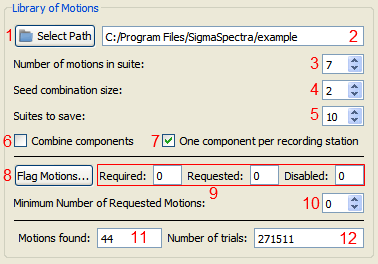
\includegraphics[scale=0.7]{screenshots/libraryOfMotions}
  \end{center}
  \caption{Screen shot of the Library of Motions Group.}
  \label{fig:interface:libraryOfMotions}
\end{figure}

The Library of Motions Group is used to specify the library of motions
considered, as well as the parameters that govern the selection procedure
described in Section~\ref{sec:method}. The fields are numbered in
Figure~\ref{fig:interface:libraryOfMotions}, and described as follows:
\begin{enumerate}
  \item Opens a dialog that is used to select the path to the folder containing
	the motions to be considered in the selection procedure. More information
	regarding collection and required organization of the input motions can be
	found in Section~\ref{sec:example:library}.
  \item Field to manually specify the file path to the motion library.
  \item The number of motions in a suite.
  \item The seed combination size. This parameter controls the number of trials
	will be performed during the selection procedure as described in
	Section~\ref{sec:method:selecting}. The larger this number is the more
	number of trials are performed.
  \item The number of suites to be saved by SigmaSpectra for consideration by
	the user. For example, if this number were 10 then the suites with the 10
	lowest RMSE values are saved.
  \item If the horizontal components from a station are to be combined prior to
	the selection process. The horizontal components ($A$ and $B$) are combined
	using the geometric mean ($\sqrt{A \cdot B}$), and then the average spectrum
	treated as single motion in the selection process. This option would be
	appropriate for analysis requiring two components of motion. The
	identification of component pairs is done using the file naming conventions
	of the PEER NGA database. This option disables the \emph{One component per
	recording station} check box.
  \item If only one component per recording station is allowed in a suite. If
	this is enabled, then suites are limited to only contain one component per
	recording station for each event.
  \item Opens the Flag Motion Dialog discussed in
	Section~\ref{sec:interface:flagMotions}.
  \item The number of the \emph{Required}, \emph{Requested}, and
	\emph{Disable} motions.
  \item The minimum number of\emph{Requested} motions in a valid suite.
  \item The number of motions found with the motion library.
  \item The number of trials that will be performed during the selection process.
\end{enumerate}

\FloatBarrier
\subsubsection{Calculation Group}
\label{sec:interface:calculation}

\begin{figure}[h]
  \begin{center}
	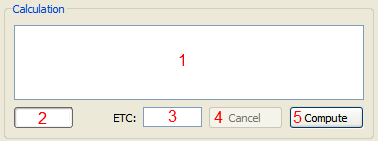
\includegraphics[scale=0.7]{screenshots/calculation}
  \end{center}
  \caption{Screen shot of the Calculation Group.}
  \label{fig:interface:calculation}
\end{figure}

The Calculation Group is used to start and cancel the selection process, as
well as report information regarding the process. The fields are numbered in
Figure~\ref{fig:interface:calculation}, and described as follows:
\begin{enumerate}
  \item Message window containing information about the status of the selection
	process.
  \item The progress of the selection process.
  \item The estimated time at which the selection of suites will be completed.
  \item The \emph{Cancel} button used to stop the selection process. Only
	enabled when the selection process is ongoing.
  \item The \emph{Compute} button used to start the selection process. After
	the selection process is completed, the Suite Selection Dialog (see
	Section~\ref{sec:interface:suiteSelection}) is displayed.
\end{enumerate}

\FloatBarrier
\subsection{Flag Motions Dialog}
\label{sec:interface:flagMotions}

\begin{figure}[h]
  \begin{center}
	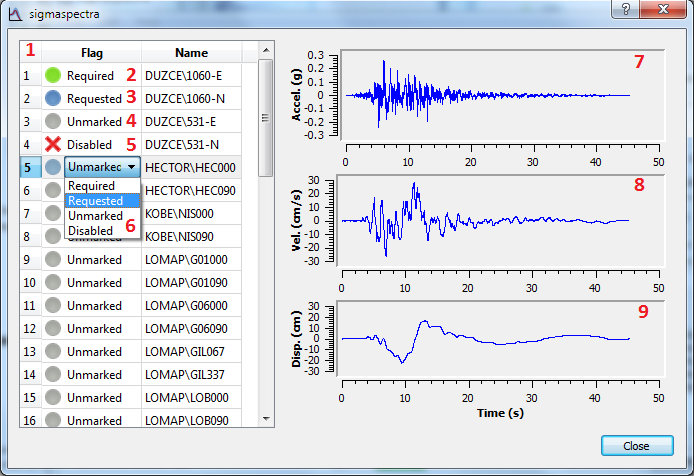
\includegraphics[scale=0.7]{screenshots/flagMotions}
  \end{center}
  \caption{Screen shot of the Flag Motions Dialog.}
  \label{fig:interface:flagMotions}
\end{figure}

The Flag Motions Dialog is an optional step that allows the user greater
control during the selection process by allowing each motion to be to flagged as
either \emph{Required}, \emph{Requested}, \emph{Unmarked} (the default state), or
\emph{Disabled}. The flags are described as follows:
\begin{description}
  \item[Required] Suite must contain the motion.
  \item[Requested] Suite must contain at least the number of \emph{Requested} motions
	defined by the Minimum Number of Requested Motions Spin Box in the
	Library of Motions Group (see \#10 in
	Figure~\ref{fig:interface:libraryOfMotions}).
  \item[Unmarked] No preference is given to the motion. This is the default
	motion flag.
  \item[Disable] Suite must not contain the motion.
\end{description}
An example of when flagging motions may be useful is when the suite should
contain a certain number of motions with directivity pulses.  The dialog is
launched by pressing button \#8 in the Library of Motions Dialog
(Figure~\ref{fig:interface:libraryOfMotions}). When the
\emph{One component per recording station} check box is enabled, then the
horizontal components are grouped together. The dialog is shown in
Figure~\ref{fig:interface:flagMotions}, and described as follows:
\begin{itemize}
  \item Table containing all motions found in the library path.
  \item A motion listed as \emph{Required}.
  \item A motion listed as \emph{Requested}.
  \item A motion listed as \emph{Unmarked}.
  \item A motion listed as \emph{Disabled}.
  \item The drop-down list used to flag the motions.
  \item Acceleration-time series of the motion(s). If the \emph{Combine
	components} check box (see \#6 in
	Figure~\ref{fig:interface:libraryOfMotions}) is enabled, then both
	components are plotted.
  \item Velocity-time series of the motion(s). If the \emph{Combine components}
	check box (see \#6 in Figure~\ref{fig:interface:libraryOfMotions}) is
	enabled, then both components are plotted.
  \item Displacement-time series of the motion(s). If the \emph{Combine
	components} check box (see \#6 in
	Figure~\ref{fig:interface:libraryOfMotions}) is enabled, then both
	components are plotted.
\end{itemize}

\subsection{Suite Selection Dialog}
\label{sec:interface:suiteSelection}

The Suite Selection Dialog is used to display information about a suite
to help the user select a suite of motions.  The components of the dialog are
shown in Figure~\ref{fig:interface:suiteSelection}, and described as follows:
\begin{enumerate}
  \item The list of suite saved during the selection procedure. The table
	consists of four columns and can be sorted by any column. The four columns
	are:
	\begin{description}
	  \item[Export] If the suite is to be exported.
	  \item[Rank] Allows the user to give the suite a numerical rank (\emph{optional}).
	  \item[Median Error] Root-mean-square-error of the median response spectrum to
		the target response spectrum.
	  \item[Stdev. Error] Root-mean-square-error of the standard deviation
		($\sigma_{\ln}$) to the target standard deviation.
	\end{description}
  \item A list of the motions in the suite and the properties of the scaled
	motion. Double-clicking on a motion opens the plots of the time series.
  \item Plot of the response spectra. The coloring is as follows:
	\begin{description}
	  \item[Red--Solid] Target median response spectrum.
	  \item[Red--Dashed] Target median response spectrum plus/minus one standard
		deviation.
	  \item[Blue--Solid] Median response spectrum of the suite.
	  \item[Blue--Dashed] Median response spectrum of the suite plus/minus one
		standard deviation.
	  \item[Green] Currently selected motion.
	  \item[Gray] Unselected motions.
	\end{description}
  \item Plot the standard deviation ($\sigma_{\ln}$). The color is as follows:
	\begin{description}
	  \item[Red--Solid] Target standard deviation.
	  \item[Blue--Solid] Suite standard deviation.
	\end{description}
  \item Plot of the acceleration-, velocity-, and displacement-time series for
	the currently selected motion.
  \item Export the selected suites (see Section~\ref{sec:interface:export})
  \item Close the dialog.
\end{enumerate}

\begin{figure}[tbp]
  \begin{center}
	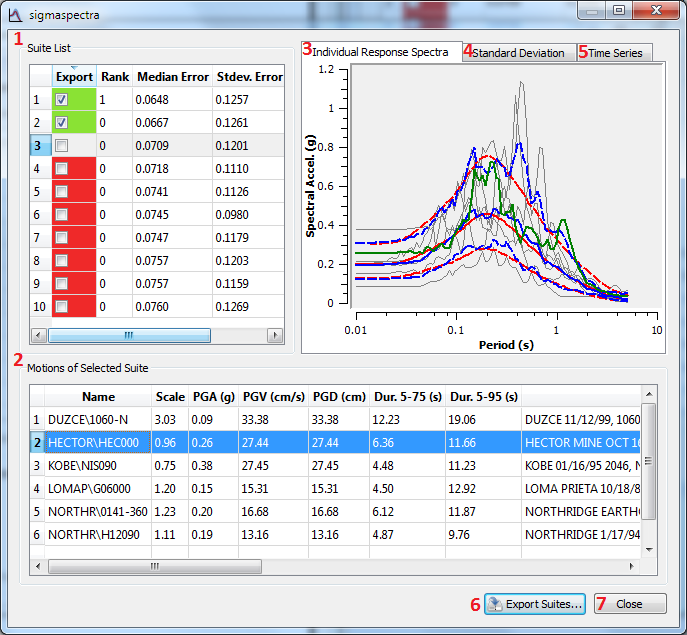
\includegraphics[width=\textwidth]{screenshots/suiteSelection}
  \end{center}
  \caption{Screen shot of the Suite Selection Dialog.}
  \label{fig:interface:suiteSelection}
\end{figure}

\subsection{Export Dialog}
\label{sec:interface:export}

A suite can be saved from the program by pressing the \emph{Export Suites...}
button (\#6 in Figure~\ref{fig:interface:suiteSelection}) which opens the
Export Dialog, shown in Figure~\ref{fig:interface:export}. The dialog
consists of the following elements:
\begin{enumerate}
  \item The output format of the selected suites:
	\begin{description}
	  \item[No Output] Nothing for each suite is written. This format option is
		only useful if the \emph{Include a summary of all generated suites}
		option (\#4 in Figure~\ref{fig:interface:export}) is also enabled.
	  \item[Comma separated values] The most complete output option, which
		includes the scaled response spectra, as well as scale factor and
		characteristics for each motion within the suite. This file can be
		easily opened with a spreadsheet program.
	  \item[Strata suite file] A file consisting of the file path and scale
		factor separated by a comma for each motion within the suite. This file
		can be open with the site response analysis program Strata.
	  \item[SHAKE2000 suite file] A file consisting of the file path and scale
		factor for each motion within the suite in a fixed width format. This file
		can be open with the site response analysis program SHAKE2000.
	\end{description}
  \item The prefix to apply to the created files (\emph{optional}).
  \item The folder where the exported files will be created.
  \item If a summary of all saved suites should be created.
  \item Write the files and close the dialog.
  \item Close the dialog without creating the files.
\end{enumerate}

\begin{figure}[tbp]
  \begin{center}
	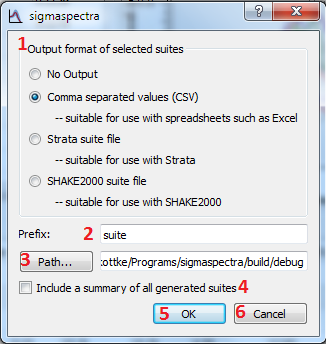
\includegraphics[scale=0.7]{screenshots/export}
  \end{center}
  \caption{Screen shot of the \emph{Export Dialog}.}
  \label{fig:interface:export}
\end{figure}

\section{An Example}
The use of SigmaSpectra can be simplified to the following five steps:
\begin{enumerate}
\item Define the scenario event and the desired number of motions in the suite.
\item Compute the target response spectrum and standard deviation for the scenario event.
\item Create a library of ground motions suitable for the scenario event.
\item Generate a number of potential suites with SigmaSpectra.
\item Select the suite(s) to be used in the analysis.
\end{enumerate}
Each of these steps will be discussed through the use of an example. This
introduction to ground motion selection is not to be considered exhaustive.

\subsection{Scenario Event}
The scenario event is usually defined by the project. In this example, the scenario event will be a
magnitude 7.0 earthquake generated by a strike-slip fault at a distance of 20 km. SigmaSpectra will
be used to generate 30 different suites, with each suite containing 10 ground motions. The size of
the suite affects the fit of both the median and the standard deviation.
%% FIXME more here


\subsection{Target Response Spectrum}
Defining a target response spectrum for a scenario event and application
requires the use of engineering judgment and will not be discussed here.
However, it is important to point out that it may not be appropriate to use
SigmaSpectra to fit every response spectrum. If the response spectrum is
representative of a threshold response, instead of a median response, then the
use of SigmaSpectra is not encouraged.

For the example scenario, the \citet{abrahamson:97} attenuation relation was
used to compute the target response spectrum and standard deviation presented in
Table~\ref{tab:target}. If the \emph{Example} option was enabled during
installation, this target response spectrum can also be opened from the
\emph{example-target.csv} file found in the installation directory. The damping
used in this in this model is 5\%. Because the limited number of periods
specified by this model, we will use an interpolated period range. Consistent
RMSE values have been found by using at least 60 steps between 0.01 and 5
seconds which corresponds to approximately 25 steps per log cycle. For this
example, we will use 100 points from 0.01 to 5 seconds.

\begin{table}[tbp]
\centering
\begin{tabular}{ccc}
\hline\hline
\textbf{Period (s)} & \textbf{Sa (g)} & \textbf{Stdev.} ($\sigma_{\ln}$) \\
\hline
0.010 & 0.19983 & 0.430 \\
0.020 & 0.19983 & 0.430 \\
0.030 & 0.21694 & 0.430 \\
0.040 & 0.24288 & 0.440 \\
0.050 & 0.26785 & 0.440 \\
0.060 & 0.28857 & 0.450 \\
0.075 & 0.31805 & 0.460 \\
0.090 & 0.33892 & 0.470 \\
0.100 & 0.35845 & 0.470 \\
0.120 & 0.39258 & 0.480 \\
0.150 & 0.43705 & 0.480 \\
0.170 & 0.45219 & 0.490 \\
0.200 & 0.45931 & 0.500 \\
0.240 & 0.44796 & 0.500 \\
0.300 & 0.41705 & 0.510 \\
0.360 & 0.38132 & 0.520 \\
0.400 & 0.36087 & 0.520 \\
0.460 & 0.32983 & 0.536 \\
0.500 & 0.30779 & 0.540 \\
0.600 & 0.27312 & 0.556 \\
0.750 & 0.22736 & 0.564 \\
0.850 & 0.20727 & 0.578 \\
1.000 & 0.18158 & 0.594 \\
1.500 & 0.12073 & 0.620 \\
2.000 & 0.08829 & 0.640 \\
3.000 & 0.04781 & 0.676 \\
4.000 & 0.02924 & 0.696 \\
5.000 & 0.02012 & 0.716 \\
\hline\hline
\end{tabular}
\caption{Target response spectrum computed using the \citet{abrahamson:97} attenuation
relationship.}
\label{tab:target}
\end{table}

\subsection{Defining a Library of Ground Motions}\label{sec:example:library}

Before a suite of ground motions can be selected, a library of potential motions
must be developed.  Care needs to be taken in the selection of ground motions
for this library. Each of the motions should be application to the scenario
characterized by the target response spectrum. Because of the challenge in
selecting appropriate motions no discussion of the subject will be presented
here.

Currently, SigmaSpectra only supports the processing of Next Generation
Attenuation (NGA) times series which can be downloaded from
\url{http://peer.berkeley.edu/nga/earthquakes.html}. The NGA database names
files based on the \emph{recording station and component only}. Therefore, two
time series from the same station and component have the same name for two
different earthquakes. In part of the NGA data organization files are stored in
directories corresponding to the earthquake event name. For example, recordings
from the Northridge earthquake are all found in the \emph{NORTHR} folder. It is
recommended that a similar convention be used for organizing files for use by
SigmaSpectra. The NGA earthquake name can be found in URL for for the ground
motion records. For example, link to download the 95$^\circ$ component recording
at the \emph{Wonderland Ave} station for the Northridge earthquake is
\emph{NORTHR/WON095} and the url:
\url{http://peer.berkeley.edu/nga\_files/ath/NORTHR/WON095.AT2}. I would
recommend saving the \emph{WON095.AT2} file to a directory named \emph{NORTHR}
to maintain organization.

For the example, a catalog of potential motions was selected by searching the
NGA strong motion database using the parameters shown in
Table~\ref{tab:motSearchSummary}. These parameters -- magnitude range, distance
range, faulting mechanism, and rock site conditions -- are specified such that a
variety of motions are present in the catalog and that each of the motions in
the catalog was generated under conditions similar to the scenario. The search
resulted in a total of 44 motions, as summarized in
Table~\ref{tab:motSearchResults}. The motions were recorded from 6 different
earthquakes with a majority (38 out of 44) of the motions being recorded for
earthquakes with a magnitude below scenario event. Because of the duration being
related to the magnitude, the limited number of motions from large magnitude
earthquakes may result in combinations with median durations that are shorter
than the expected duration of the scenario. If duration were critical in the
analysis, the upper limit on the magnitude range could be extended to include
more motions with longer durations.   

\begin{table}[tb]
  \centering
  \begin{tabular}{lcc}
	\hline\hline
	\textbf{Parameter} & \textbf{Values}\\
	\hline
	Magnitude ($M_w$)		& 6.6 to 7.3 \\
	Closest Distance		& 5 to 30 km \\
	Fault Type				& Strike-Slip, Reverse \\
	$V_{s,30}$				& 600 to 2500 m/s \\
	GeoMatrix 1 Class		& A, B, and I \\
	\hline\hline
  \end{tabular}
  \caption{Parameters used to define motions for consideration in the selection algorithm.}
  \label{tab:motSearchSummary}
\end{table}

\begin{table}[tb]
  \centering
  \begin{tabular}{lllc}
	\hline\hline
	\textbf{Event} & \textbf{Magnitude} & \textbf{Fault Type} & \textbf{No. of Records} \\
	\hline
	San Fernando			& 6.61	& Reverse 			& 6 \\
	Northridge				& 6.69	& Reverse			& 18 \\
	Kobe, Japan				& 6.9	& Strike-Slip		& 2 \\
	Loma Prieta				& 6.93	& Reverse-oblique	& 12 \\
	Hector Mine				& 7.13  & Reverse			& 2 \\
	Duzce, Turkey 			& 7.14	& Strike-Slip		& 4 \\
	\hline\hline
  \end{tabular}
  \caption{The earthquake events and number of records used in the catalog of motions.}
  \label{tab:motSearchResults}
\end{table}

During the installation the motions for this scenario can be installed by
selecting the \emph{Example} option. The motions are then installed into the
\emph{example} folder of the installation path. Select this folder by clicking
on \emph{Select Path} and selecting the appropriate folder, or by typing in
the appropriate path. Once the path is specified, the \emph{Motions found} box
will update with the number of motions recursively found within the specified
directory. At this time the number of motions in the suite, seed combination
size, and suites to save can all be defined.

Ground motions are recorded at stations and for each event there are three
components of recorded (two horizontal and one vertical). The horizontal
components are used in most applications, and are the only components that are
loaded by SigmaSpectra. The horizontal components for a given event and station
are related to each other. In some cases, it might not be appropriate to create
a suite that contains both horizontal components for the same station and event.
To limit the suite to only one component per recording station, check the
\emph{One component per recording station} check box. In other cases, such as
two-dimensional analysis, the user might want to select pairs of components.
This feature is enabled by checking the \emph{Combined components} check box.
The components are combined in log-space, and the station is then selected
instead of the components during the selection process, and the same scale
factor is applied to each component.

\subsection{Generate Potential Suites}

Once the library of the of ground motions has been developed, the parameters for
used in the suite selection process need to be defined. The parameters used in
this example are tabulated in Table~\ref{tab:example:selectionParams}. The
number of motions in the suite is dependent on the project; for this example
ground motion suite will consist of seven motions. The seed combination size is
used to adjust how rigorous the search procedure is for the selection of the
ground motion suites. If the seed combination size is the same as the number of
motions in a suite, then every possible combinations of motions will be tried,
but will take a very long time (possibly days to weeks).  For most cases, a seed
of two or three is appropriate. The motions are being selected for a one
dimensional analysis (i.e., components will not be combined). Only one motion
per recording station is allowed so that the path effect captured by each motion
is independent of the other motions in the suite.

\begin{table}
  \centering
  \begin{tabular}{lc}
	\hline\hline
	\textbf{Option} & \textbf{Value}\\
	\hline
	Number of motions in suite & 7 \\
	Seed combination size & 2 \\
	Suites to save & 10 \\
	Combined components & No \\
	One component per recording station & Yes \\
	\hline\hline
  \end{tabular}
  \caption{Example selection parameters.}
  \label{tab:example:selectionParams}
\end{table}

After fully defining the target response spectrum, ground motion library, and
parameters governing the selection process press the \emph{Compute} button to
start the automated-selection process. Once the suites have been selected, a new
will be created with the potential suites to allow the user to make the final
decision.

\subsection{Selection of Suites}

Selection of the final suite(s) requires use of engineering judgment. The user
may want to consider the fit of the selected motions to the target response
spectrum at various periods, the variability of the suite, and characteristics
of the time series. If is suite is deemed to be appropriate, then it is enabled
for export in the Suite List Table (\#1 in
Figure~\ref{fig:interface:suiteSelection}).

Suites that have been marked for export are exported with the \emph{Export}
button. The suite can be exported in a variety of formats. The most general use
is the comma-separated values format as it also includes the response spectra of
each ground motion in the suite. Each suite is exported to a different file
name, the prefix of which can be specified.

\bibliography{references}

\subsection{Ground Motion Format}

SigmaSpectra was developed to use ground motions retrieved from the Pacific
Earthquake Engineering Research (PEER) Center database. Motions not included in
the PEER database can be considered if they are first transformed into the AT2
format. The following guidelines must be followed:
\begin{itemize}
    \item The file extension must be ``AT2''. Note that the test on the file
      extension is case sensitive so ``at2'' is not acceptable.
    \item Header lines:
      \begin{description}
        \item[Line 1] Not used
        \item[Line 2] Detailed description of the motion (optional).
        \item[Line 3] Not used
        \item[Line 4] Number of data points and time step separated by
          whitespace (e.g., \texttt{2048 0.01})
      \end{description}
    \item Acceleration data format can be either single or multiple points per
      line. Only the number of points specified in header line 4 is read. The
      acceleration values must be specified in units of gravity.
\end{itemize}

\end{document}
